\section{Normalization of \acs*{dce}-\acs*{mri} images}\label{sec:chp5:DCE-norm}

This section focuses on \ac{dce}-\ac{mri} normalization.
We recall that in \ac{dce}-\ac{mri}, a contrast media is injected intravenously and a set of images is acquired over time.
Consequently, each voxel in an image corresponds to a dynamic signal which is related to both contrast agent concentration and the vascular properties of the tissue.
Therefore, changes of the enhanced signal allows to discriminate healthy from \ac{cap} tissues.
In fact, these properties are automatically extracted using quantitative or semi-quantitative approaches~\cite{Lemaitre2015}.

\emph{Quantitative} approaches uses pharmacokinetic modelling based on a bicompartment model, namely Brix~\cite{brix1991pharmacokinetic} and Tofts~\cite{tofts1995quantitative} models.
The parameters of the Brix model are inferred assuming a linear relationship between the media concentration and the \ac{mri} signal intensity.
This assumption has shown, however, to lead to inaccurately estimate the pharmacokinetic parameters~\cite{heilmann2006determination}.
Instead, the Tofts model requires a conversion from the \ac{mri} signal intensity to concentration, which becomes a non-linear relationship using the specific equations of the \ac{mri} sequences (e.g., FLASH sequence).
Tofts modelling suffers, however, from a higher complexity~\cite{gliozzi2011phenomenological}.
Indeed, the conversion using the non-linear approach requires to acquire a T$_1$ map which is not always possible during clinical examination.
Additionally, the parameter calculation requires the \ac{aif} which is challenging to measure and can also lead to an inaccurate estimation.

\emph{Semi-quantitative} approaches are rather mathematical than pharmacokinetic modelling since no pharmacokinetic assumption regarding the relation between the \ac{mri} signal and the contrast agent are made~\cite{huisman2001accurate,gliozzi2011phenomenological}.
These methods offer the advantages to not require any knowledge about the \ac{mri} sequence nor any conversion from signal intensity to concentration.
However, they present some limitations: the heuristic approach proposed by \citeauthor{huisman2001accurate}~\cite{huisman2001accurate} requires an initial estimate of the noise standard deviation of the signal as well as some manual tuning.

Nevertheless, all presented methods suffer from 2 major drawbacks:
(i) inter-patient variability and (ii) loss of information.
The inter-patient variability is mainly due to the acquisition process and consequently leads to generalization issue while applying a machine learning algorithm.
All previous methods extract few discriminative parameters to describe the \ac{dce}-\ac{mri} signal which might lead to a loss of information.
%(i) the inter-patient variability of the data lead to a variation of the parameters estimated and subsequently to poor classification performance while designing \ac{cad} systems, and
%(ii) only few parameters are used to characterize the dynamic signal implying that some information are discarded.

In this section, we propose a fully automatic normalization method for \ac{dce}-\ac{mri} that reduces the inter-patient variability of the data.
The benefit and simplicity of our approach will be shown by classifying the whole normalized \ac{dce}-\ac{mri} signal and comparing with the state-of-the-art quantitative and semi-quantitative methods.
Additionally, we will show that using this normalization approach in conjunction with the quantitative methods improves the classification performance of most of the models.
We also propose a new clustering-based method to segment enhanced signals from the arteries, later used to estimate an \ac{aif} as well as an alternative approach to estimate the parameters of the semi-quantitative model proposed by~\cite{huisman2001accurate}.

% The benefit of our approach will be shown while using quantitative and semi-quantitative approaches.
% Additionally, we show that using the whole normalized \ac{dce}-\ac{mri} signal is preferable to quantitative and semi-quantitative methods, leading to the best classification performance.

This section is organized as follows:
First, \acs{sec}\,\ref{subsubsec:chp5:DCE-norm:norm} details our normalization strategy for \ac{dce}-\ac{mri} data.
Quantitative and semi-quantitative methods are summarized in \acs{sec}\,\ref{subsubsec:chp5:DCE-norm:stateart} with insights about their implementations.
Finally experiments and results to answer the previous stated challenges are reported in \acs{sec}\,\ref{subsec:chp5:DCE-norm:exp-res} while discussed in \acs{sec}\,\ref{subsec:chp5:DCE-norm:dis-con}, followed by a concluding section.
%Section~\ref{sec:methods} outlines our normalization strategy (Section~\ref{sec:norm}) as well as specificity regarding the state-of-the-art methods used for comparison (Section~\ref{sec:stateart}).
%The dataset, experiments, and results are reported in Section~\ref{sec:experiments} while discussed in Section~\ref{sec:discussions} followed by a concluding section.


\subsection{Methodology} \label{subsec:chp5:DCE-norm:meth}

\subsubsection{Normalization of \ac{dce}-\ac{mri} images}\label{subsubsec:chp5:DCE-norm:norm}

\begin{figure}
  \centering
  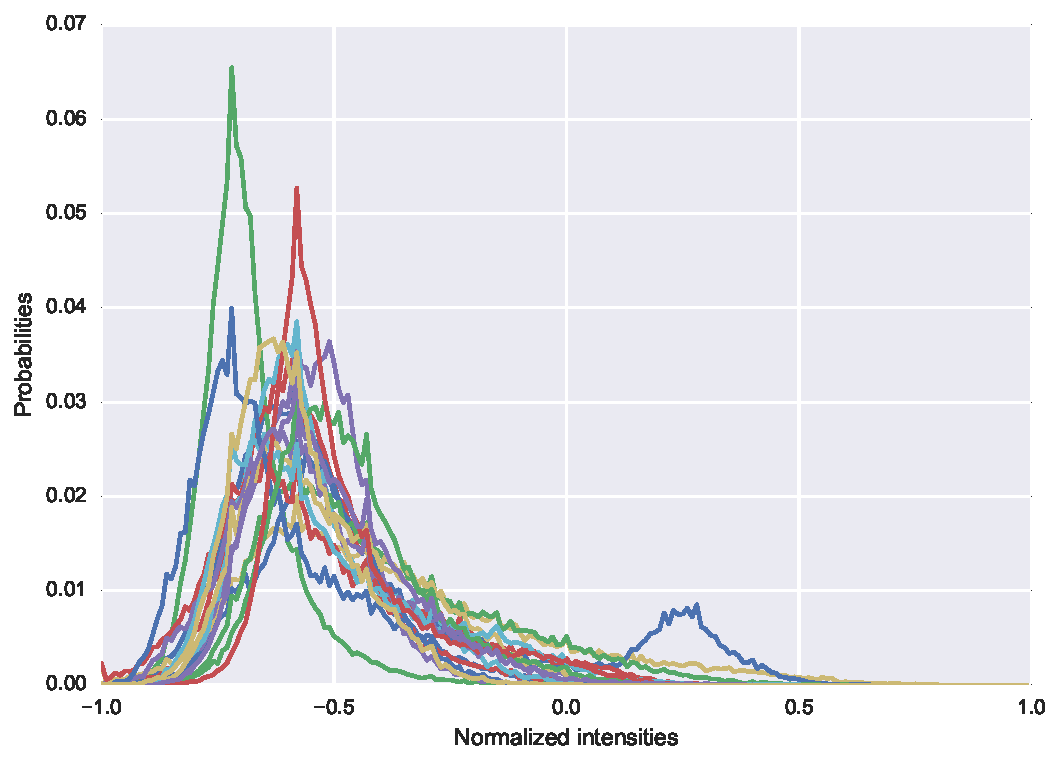
\includegraphics[width=0.7\linewidth]{5_normalization/figures/DCE-normalization/t2wImage.pdf}
  \caption{Illustration of the inter-patient variations in 17 different patients, using the \acs*{pdf} representation.}
  \label{fig:t2}
\end{figure}

In this section, we propose a method to normalize \ac{dce}-\ac{mri} prostate data to reduce inter-patient variations, although it can be applied to any \ac{dce}-\ac{mri} sequences.
As presented in the previous section, in \ac{t2w}-\ac{mri}, these variations are characterized by a shift and a scaling of the intensities as illustrated by the intensity \ac{pdf} in \acs{fig}\,\ref{fig:t2}.
Therefore, these variations can be corrected using a $z$-score approach --- i.e., normalizing the data by subtracting the mean and dividing by the standard deviation --- assuming that the data follow a specific distribution~\cite{lemaitre2016normalization}.

\begin{figure}
  \centering
  \hspace*{\fill}
  \subfigure[]{\label{subfig:pathhist}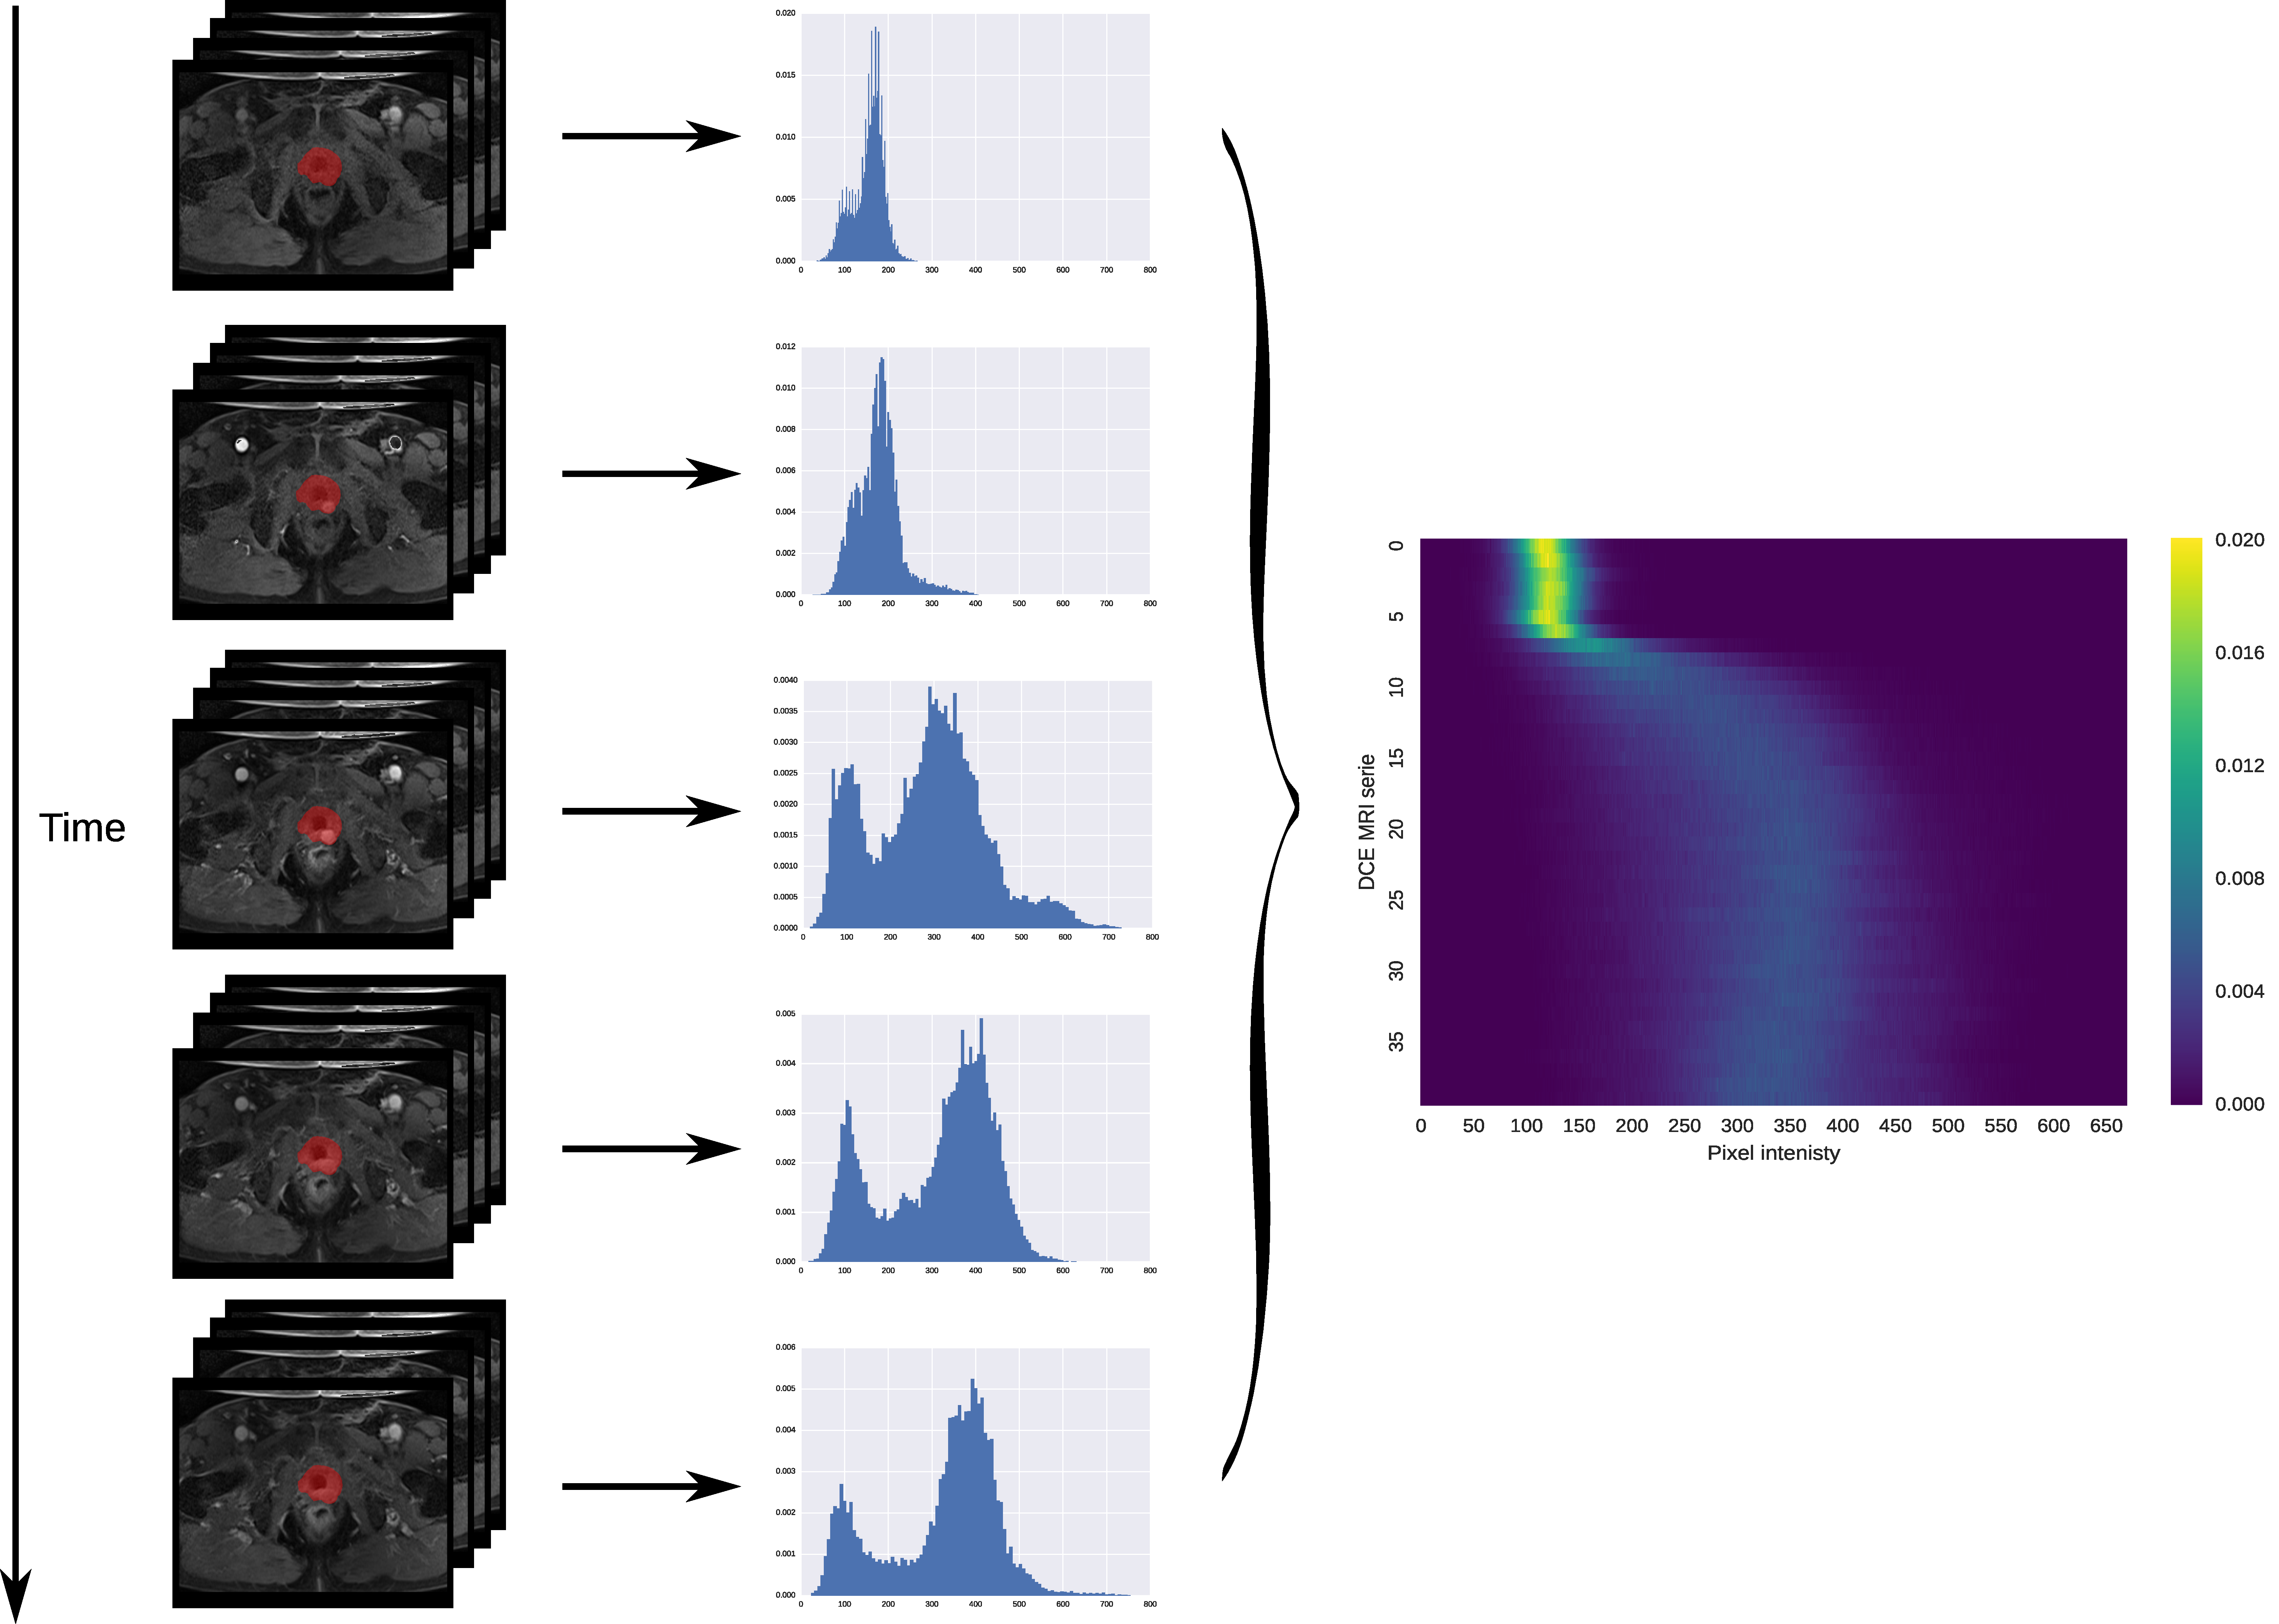
\includegraphics[width=1\textwidth]{5_normalization/figures/DCE-normalization/heatmaprep.pdf}} \hfill
  \hspace*{\fill}
  \\
  \hspace*{\fill}
  \subfigure[]{\label{subfig:pat1}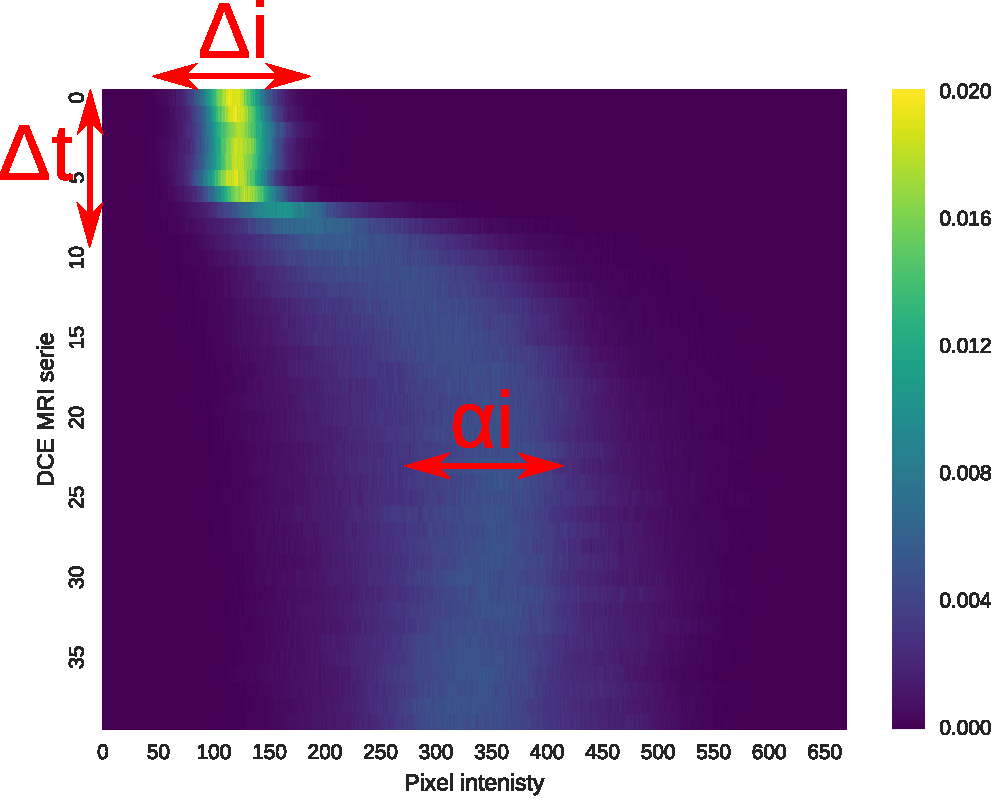
\includegraphics[width=.49\textwidth]{5_normalization/figures/DCE-normalization/pat1_annotated.pdf}} \hfill
  \subfigure[]{\label{subfig:pat2}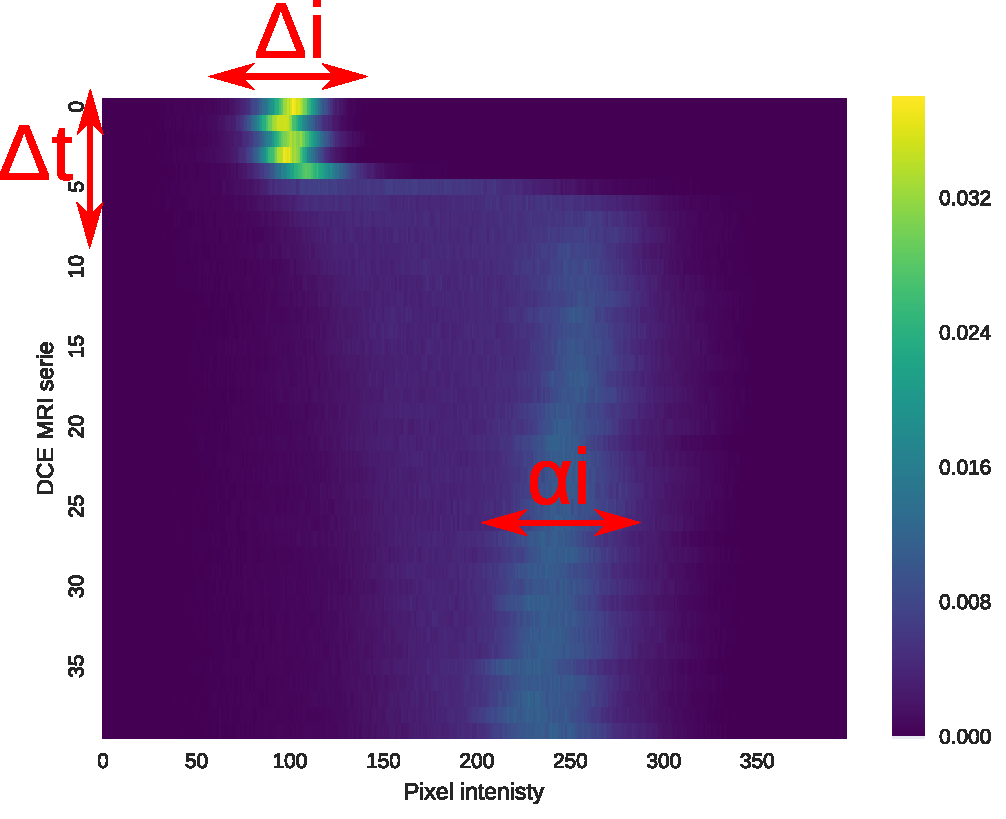
\includegraphics[width=.49\textwidth]{5_normalization/figures/DCE-normalization/pat2_annotated.pdf}} \hfill
  \hspace*{\fill}
  \caption[Illustration of the heatmap in \acs*{dce}-\acs*{mri} images.]{\ac{dce} normalization: \subref{subfig:pathhist} Illustration of the heatmap representation: all \acs*{pdf}s of the prostate gland are concatenated together to build an heatmap; \subref{subfig:pat1}-\subref{subfig:pat2} Illustration of inter-patient variations (i.e., $\Delta_i$, $\Delta_t$, and $\alpha_i$) \acs*{pdf} over time of two patients in a \acs*{dce}-\acs*{mri}.}
  \label{fig:heatmap}
\end{figure}

In \ac{dce}-\ac{mri}, the intensity \ac{pdf} of prostate gland does not follow a unique type of distribution such as Rician or Gaussian distribution, as shown in \acs{fig}\,\ref{subfig:pathhist}.
Indeed, the inter-patient variations are more complex due to the temporal acquisition.
A better representation to observe these variations is to represent the intensity \ac{pdf} of the prostate gland over time --- requiring to segment the prostate --- using a heatmap representation as shown in \acs{fig}\,\ref{subfig:pathhist}.
Analyzing this heatmap representation across patients (see Fig.\,\ref{subfig:pat2}), the following variations are highlighted:
(i) intensity offsets $\Delta_i$ of the \ac{pdf} peak,
(ii) a time offset $\Delta_t$ depending of the contrast agent arrival, and
(iii) a change of scale $\alpha_i$ related to the signal enhancement.
Therefore, our normalization method should attenuate all these variations and be performed globally across the different time sequences rather than for each independent sequence.

\paragraph{Graph-based intensity offsets correction}\label{par:chp5:DCE-norm:graph}

\begin{figure}
  \centering
  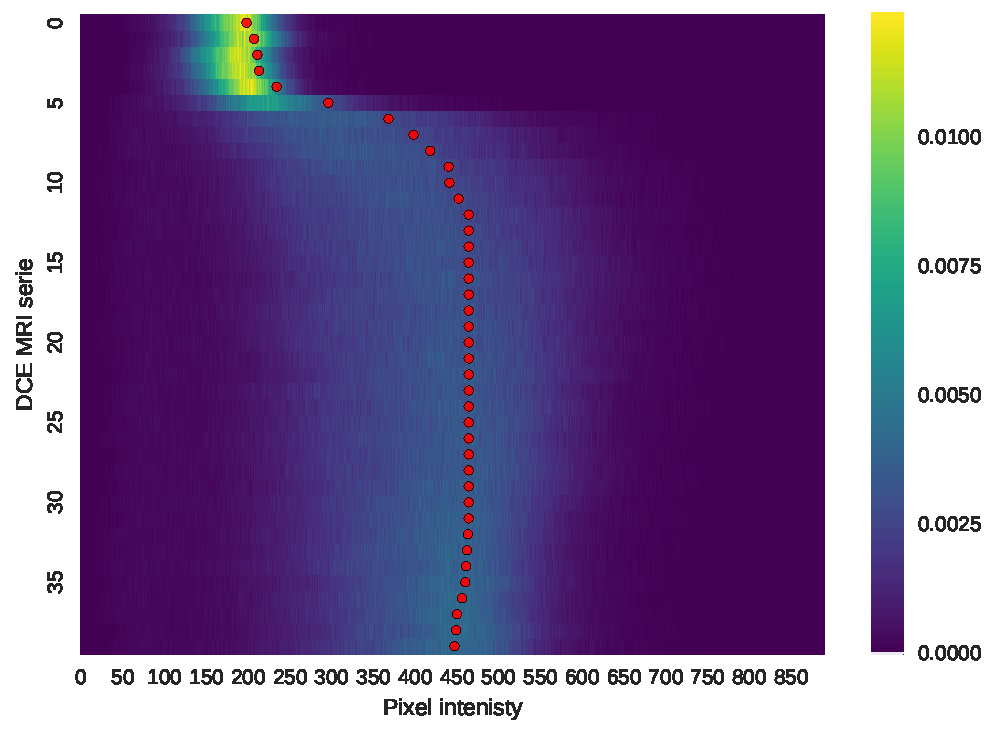
\includegraphics[width=0.7\linewidth]{5_normalization/figures/DCE-normalization/estimator.pdf}
  \caption{Illustration of the estimator found using the shortest-path through the graph.}
  \label{fig:estimator}
\end{figure}

Before to standardize each sequence, the first step of the normalization is to cancel the intensity specific at each patient, occurring due to the media injection.
As previously mentioned, the intensity \ac{pdf} does not always follow either a Rician or a Gaussian distribution over time, in \ac{dce}-\ac{mri}.
Therefore, the mean of these distributions cannot be used as a potential estimate for these offsets.
Additionally, these offsets should be characterized by a smooth transition between series over time.
Thus, this problem is solved using the graph-theory: considering the intensity \ac{pdf} over time as shown in \acs{fig}\,\ref{subfig:pathhist}, the offsets correspond to the boundary splitting the heatmap in two partitions such that they are as close as possible to the peak of the intensity \ac{pdf}, as depicted in \acs{fig}\,\ref{fig:estimator}.
Given the heatmap, a directed weighted graph $\mathcal{G}=(\mathcal{V}, \mathcal{E})$ is built by taking each bar --- i.e., the probability for a given time and pixel intensity --- of the heatmap as a node and connecting each pair of bars by an edge.
The edge weight $w_{ij}$ between 2 nodes $i$ and $j$ corresponding to 2 pixels at position $(x_i, y_i)$ and $(x_j, y_j)$, respectively, is defined as in \acs{eq}\,\eqref{eq:weight}:

\begin{equation}
  w_{ij} = \begin{cases}
    \alpha \exp(1 - \frac{H(i)}{\max(H)})       & \text{if } x_j = x_i + 1 \text{ and } y_j = y_i, \\
    (1 - \alpha) \exp(1 - \frac{H(i)}{\max(H)}) & \text{if } x_j = x_i \text{ and } y_j = y_i + 1, \\
    0                                           & \text{otherwise},
  \end{cases}
  \label{eq:weight}
\end{equation}

\noindent where $H$ is the heatmap, $\alpha$ is a smoothing parameter controlling the partitioning.

Therefore, these offsets related to $\Delta_i$ are estimated by finding the shortest-path to cross the graph using Dijkstra's algorithm.
The entry and exiting nodes are set to be the bin with the maximum probability for the first \ac{dce}-\ac{mri} serie and the bin corresponding to the median value for the last \ac{dce}-\ac{mri} serie, respectively.
To ensure a robust estimation of these offsets, the process of finding the shortest-path is repeated in an iterative manner by shifting the data and updating the heatmap as well as the graph $\mathcal{G}$.
The procedure is stopped once the offset found does not change.
In general, this process is not repeated more than 3 iterations.
The parameter $\alpha$ is set to $0.9$, empirically.
Figure~\ref{fig:estimator} illustrates the final estimation of the offsets $\Delta_i$ (i.e., red landmark) found for each \ac{dce}-\ac{mri} serie.
Therefore, each intensity offset is subtracted for each \ac{dce}-\ac{mri}.

\paragraph{Time offset and data dispersion correction}\label{par:chp5:DCE-norm:time-off}

\begin{figure}
  \centering
  \hspace*{\fill}
  \subfigure[\acs*{rmse} computed for each patient of our dataset.]{\label{fig:rmse}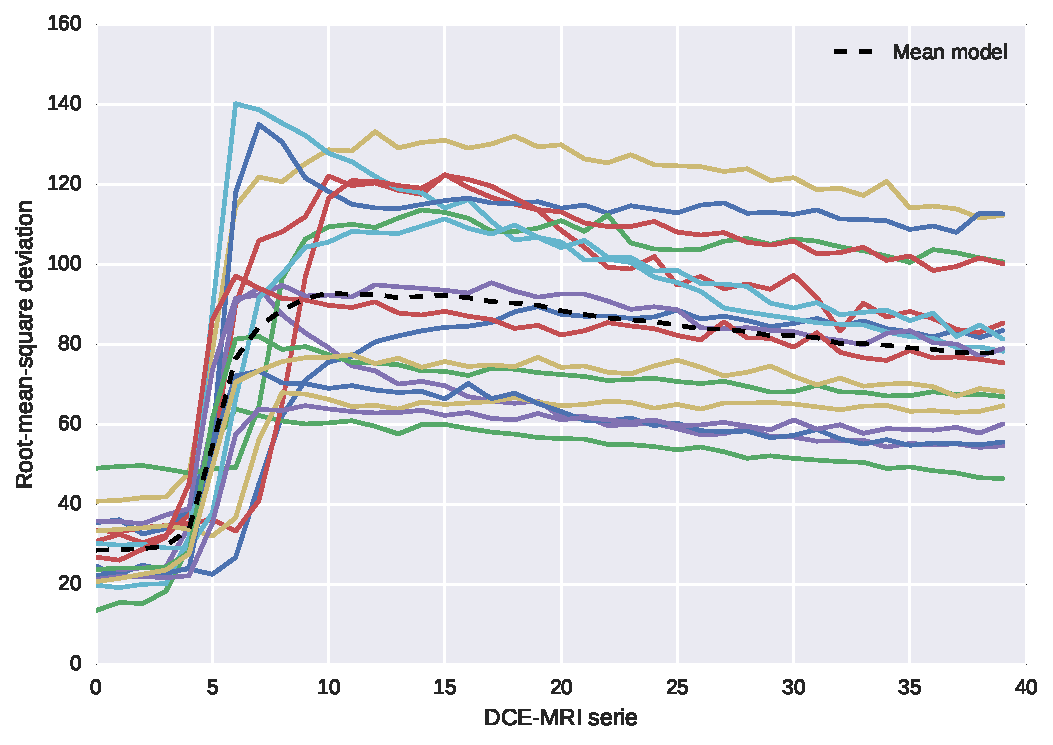
\includegraphics[width=.49\textwidth]{5_normalization/figures/DCE-normalization/rmse.pdf}} \hfill
  \subfigure[\acs*{rmse} after alignment using the curve parametric model.]{\label{fig:rmseal}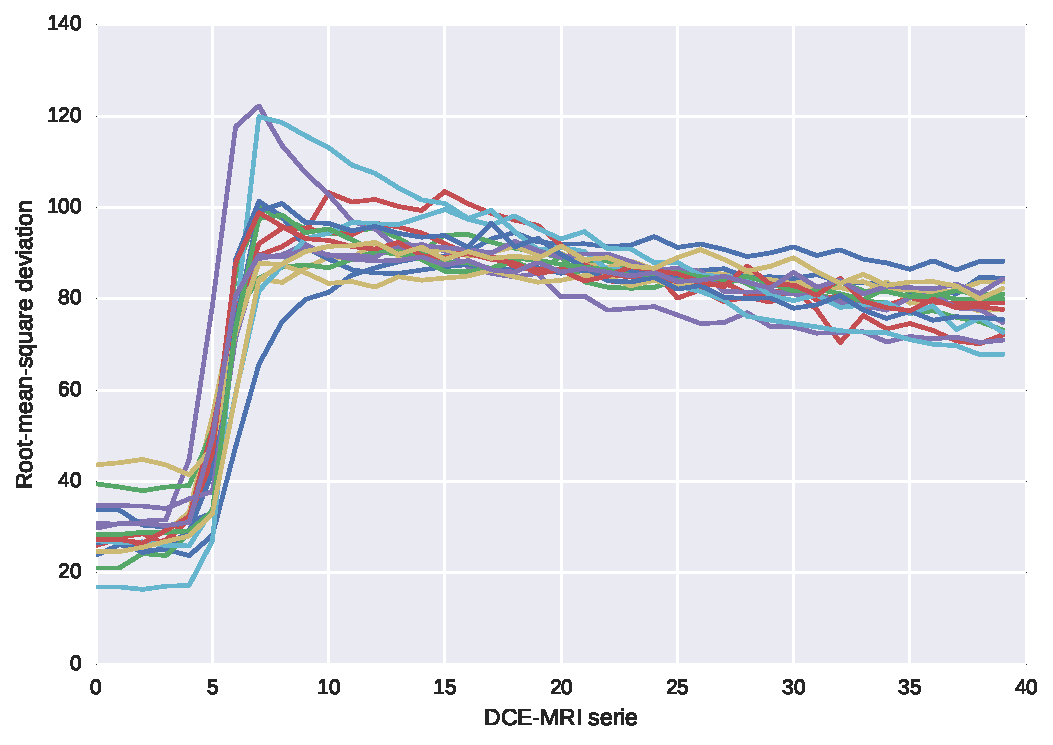
\includegraphics[width=.49\textwidth]{5_normalization/figures/DCE-normalization/rmse_aligned.pdf}}
  \hspace*{\fill}
  \caption{Illustration of the correction of the time offset and the data dispersion.}
  \label{fig:curveal}
\end{figure}

The next variations to correct are the time offset $\Delta_t$ and the data dispersion $\sigma_i$.
By computing the \ac{rmse} of the intensities for each \ac{dce}-\ac{mri} serie, one can observe these two variations as shown in \acs{fig}\,\ref{fig:rmse}.
Therefore, to correct these variations, we propose to register each patient \ac{rmse} to a mean model which corresponds to the mean of all patients \ac{rmse}.
The parametric model to perform the registration is formulated as in \acs{eq}\,\eqref{eq:model}:

\begin{equation}
  T(\alpha, \tau, f(t)) = \alpha f(t - \tau) ,
  \label{eq:model}
\end{equation}

\noindent where $\tau$ and $\alpha$ are the two parameters handling the time offset $\Delta_i$ and global scale $\sigma_i$, respectively, $f(\cdot)$ is the \ac{rmse} function defined as:

\begin{equation}
  f(t) = \sqrt{ \left( \frac{\sum_{n=1}^{N} x(t)_{n}^2}{N}  \right) },
  \label{eq:rmsd}
\end{equation}

\noindent where $x(t)_n$ is the shifted intensity of a sample from a specific \ac{dce}-\ac{mri} serie at time $t$ from a total number of $N$ samples.

Therefore the registration problem is equivalent to:

\begin{equation}
  \argmin_{\alpha, \tau} = \sum_{t=1}^{N} \left[ T\left(\alpha, \tau, f(t)\right) - \mu(t) \right]^{2} ,
  \label{eq:cost}
\end{equation}

\noindent where $\mu(\cdot)$ is the mean model, $N$ is the number of \ac{dce}-\ac{mri} serie.

Illustration of the correction applied to each \ac{rmse} patient is shown in \acs{fig}\,\ref{fig:rmseal}.
Once all these parameters have been inferred, the data are shifted as well as scaled.

The resulting normalized data can be used into 2 fashions: (i) each normalized signal can be used as a whole to determine whether the corresponding voxel is healthy or cancerous or (ii) the normalized data can be fitted using a quantitative method, as presented in the next section.
%However, for the second strategy, this is necessary to apply common intensity offsets such that the data follow a shape as expected by the different quantitative models.
%The set of offsets applied is in fact corresponding to the maximum offsets found in Sect.\,\ref{sec:intoffsets}.

\subsubsection{Quantification of \acs*{dce}-\acs*{mri}}\label{subsubsec:chp5:DCE-norm:stateart}

The quantitative approaches for detection of \ac{dce}-based features have been briefly discussed in \acs{sec}\,\ref{subsubsec:chp3:img-clas:CADX-fea-dec:DCE-fea}.
In this section, we present in details the different methods which have been used for the quantification of \ac{dce}-\ac{mri} for \ac{cap} detection~\cite{Lemaitre2015} and which will be used for comparison in this work.
Furthermore, we would like to emphasize the following additional contributions for this section: (i) a novel automatic \ac{aif} estimation algorithm based on clustering and (ii) a simplified semi-quantitative method using constrained optimization.

\paragraph{Brix and Hoffmann models}\label{par:chp5:DCE-norm:brixhoffmann}

In the Brix model~\cite{brix1991pharmacokinetic}, the \ac{mri} signal intensity is assumed to be proportional to the media concentration.
Therefore, the model is expressed as in \acs{eq}\,\eqref{eq:brix} (see also \acs{eq}\,\eqref{eq:brixmod}):

\begin{equation}
  s_n(t) = 1 + A \left[ \frac{\exp(k_{el} t') - 1}{k_{ep}(k_{ep} - k_{el})} \exp(- k_{el} t) - \frac{\exp(k_{ep} t') - 1}{k_{el}(k_{ep} - k_{el})} \exp(- k_{ep} t) \right],
  \label{eq:brix}
\end{equation}

\noindent with

\begin{equation}
  s_n(t) = \frac{s(t)}{S_0},
  \label{eq:enh}
\end{equation}

\noindent where $s(t)$ and $S_0$ are the \ac{mri} signal intensity at time $t$ and the average pre-contrast \ac{mri} signal intensity, respectively; $A$, $k_{el}$, and $k_{ep}$ are the constant proportional to the transfer constant, the diffusion rate constant, and the rate constant, respectively.
Additionally, $t'$ is set such that $0 \leq t \leq \tau$, $t' = t$ and afterwards while $t > \tau$, $t' = \tau$.

\citeauthor{hoffmann1995pharmacokinetic}~\cite{hoffmann1995pharmacokinetic} proposed a similar model as expressed in \acs{eq}\,\eqref{eq:hoffmann}, which derive from the Brix model:

\begin{equation}
  \small
  s_n(t) = 1 + \frac{A}{\tau} \left[ \frac{k_{ep} \left( \exp(k_{el} t') - 1 \right)}{k_{el}(k_{ep} - k_{el})} \exp(- k_{el} t) - \frac{\exp(k_{ep} t') - 1}{(k_{ep} - k_{el})} \exp(- k_{ep} t) \right] ,
  \label{eq:hoffmann}
\end{equation}

\noindent in which the constant $A$ is redefined by isolating the parameter $\tau$.

The parameters $A$, $k_{el}$, and $k_{ep}$ are estimated by fitting the model using non-linear least-squares optimization solved with Levenberg-Marquardt.

\paragraph{Tofts model}\label{par:chp5:DCE-norm:tofts}

The extended Tofts model is formulated as in \acs{eq}\,\eqref{eq:exttofts} (see also \acs{eq}\,\eqref{eq:tofts}):

\begin{equation}
  C_t(t) = K_{trans} C_p(t) \Conv \exp(-k_{ep}t) + v_p C_p(t),
  \label{eq:exttofts}
\end{equation}

\noindent where $\Conv$ is the convolution operator; $C_t(t)$ and $C_p(t)$ are the concentrations of contrast agent in the tissue and in the plasma, respectively; $K_{trans}$, $k_{ep}$, and $v_p$ are the volume transfer constant, the diffusion rate constant, and the plasma volume fraction, respectively.

Therefore, Tofts model requires to:
(i) detect candidate voxels from the femoral or iliac arteries and estimate a patient-based \ac{aif} signal,
(ii) convert the \ac{mri} signal intensity (i.e., \ac{aif} and dynamic signal) to a concentration, and
(iii) in the case of a population-based \ac{aif}, estimate an \ac{aif} signal.

\begin{figure}
  \centering
  \hspace*{\fill}
  \subfigure[Original image.]{\label{fig:org}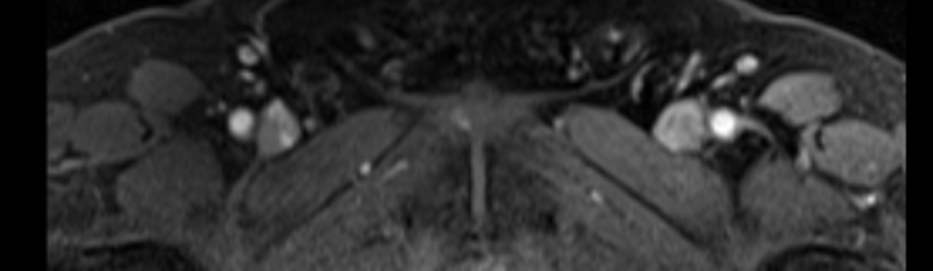
\includegraphics[width=.3\textwidth]{5_normalization/figures/DCE-normalization/original.pdf}} \hfill
  \subfigure[Candidates region after clustering.]{\label{fig:cand}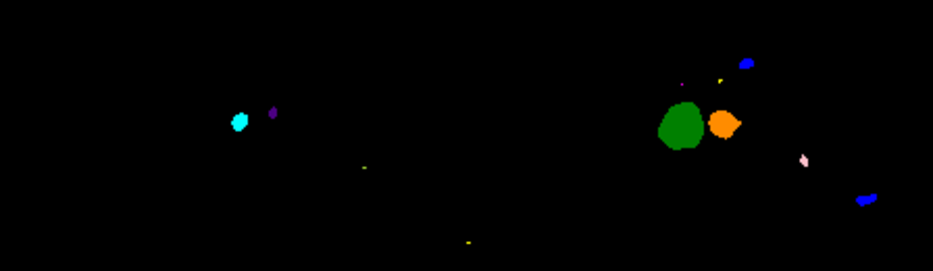
\includegraphics[width=.3\textwidth]{5_normalization/figures/DCE-normalization/candidate.pdf}} \hfill
  \subfigure[Regions selected after applying the different criteria.]{\label{fig:final}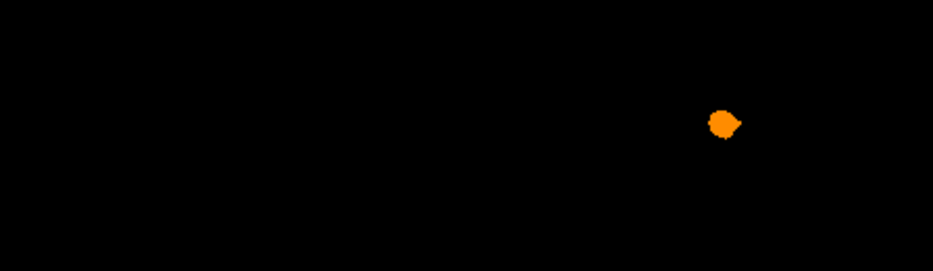
\includegraphics[width=.3\textwidth]{5_normalization/figures/DCE-normalization/aif.pdf}}
  \hspace*{\fill}
  \caption{Illustration of the segmentation of the area used to determine the \acs*{aif}.}
  \label{fig:aif}
\end{figure}

\begin{description}
  \item[Segmentation of artery voxels and patient-based \ac{aif} estimation] The \ac{aif} signal from \ac{dce}-\ac{mri} can be manually estimated by selecting the most-enhanced voxels from the femoral or iliac arteries~\cite{meng2010comparison}.
    Few methods have been proposed to address the automated extraction of \ac{aif} signal.
    \citeauthor{Chen2008} filtered successively the possible candidates to be considered as \ac{aif} such that~\cite{Chen2008}:
    (i) dynamic signals with small peak and voxels with a small wash-in are rejected by thresholding,
    (ii) a blob detector is used and large enough regions are kept, and
    (iii) circular and cylindricality criteria are used to reject the false positives.
    \citeauthor{zhu2011automated} proposed an iterative method selecting voxels which best fit a gamma variate function~\cite{zhu2011automated}.
    However, it requires to compute first and second derivatives as well as maximum curvature points.
    \citeauthor{shanbhag2012generalized} proposed a 4-steps algorithm~\cite{shanbhag2012generalized,fennessy2015quantitative}:
    (i) remove slices with artifacts and find the best slices based on intrinsic anatomic landmarks and enhancement characteristics,
    (ii) find the voxel candidates using the maximum enhanced voxels and a multi-label maximum entropy based thresholding algorithm,
    (iii) exclude region next to the endorectal coil, and
    (iv) select the best 5 candidates which meet enhancement characteristics and that are correlated.

    All the above methods are rather complex compromising robustness and generalization.
    Thus, we propose a simpler method which is based on the following reasonable assumptions:
    (i) all possible \ac{aif} signal candidates should have a similar shape,
    (ii) a high enhancement, and
    (iii) the arteries should be almost round and within a size range.
    Therefore, each slice is clustered into regions using K-means clustering with $k=6$.
    The cluster made of the most enhanced signals is selected since it contains the artery signals.
    In this regard, the selection criteria corresponds to the 90\textsuperscript{th} percentile of the maximum \ac{dce}-\ac{mri} signal.
    Finally, regions with an eccentricity smaller than $0.5$ and an area in the range of $[100, 400]$ voxels are kept.
    Additionally, to remove voxels contaminated by partial volume effect, only the \SI{10}{\percent} most enhanced voxels of the possible candidates are kept as proposed by~\cite{schabel2008uncertainty} and the average signal is computed.
    A summary of the different segmentation steps is presented in \acs{fig}\,\ref{fig:aif}.
    \item[Conversion of \ac{mri} signal intensity to concentration] To estimate the free parameters of the Tofts model (see \acs{eq}\,\eqref{eq:exttofts}), the concentration $C_t(t)$ and $C_p(t)$ need to be computed from the \ac{mri} signal intensity and the \ac{aif} signal, respectively.
      This conversion is based on the equation of the FLASH sequence --- see~\ref{app:signaltoconc} for details --- and is formulated as in Eq.\,\eqref{eq:conv}:
      \begin{equation}
        c(t) = \frac{1}{TR \cdot r_1} \ln\left( \frac{1 - \cos \alpha \cdot S^{*}\frac{s(t)}{S_0}}{1 - S^{*}\frac{s(t)}{S_0}} \right) - \frac{R_{10}}{r_1} ,
        \label{eq:conv}
      \end{equation}
      \noindent with,
      \begin{equation}
        S^{*} = \frac{1 - \exp(- TR \cdot R_{10})}{1 - \cos \alpha \cdot \exp(- TR \cdot R_{10})} ,
        \label{eq:sstarconv}
      \end{equation}
      \noindent where $s(t)$ is the \ac{mri} signal, $S_0$ is the \ac{mri} signal prior to the injection of the contrast media, $\alpha$ is the flip angle, $TR$ is the \acf{tr}, $R_{10}$ is the pre-contrast tissue relaxation time also equal to $\frac{1}{T_{10}}$, and $r_1$ is the relaxitivity coefficient of the contrast agent.

      $T_{10}$ can be estimated from the acquisition of a T$_1$ map.
      However, this modality is not part of the clinical trial in this research and the value of $T_{10}$ is fixed to \SI{1600}{\ms} for both blood and prostate, in accordance with the values found in the literature~\cite{fennessy2015quantitative,de2004mr,carr2011magnetic}.
      \item[Estimation of population-based \ac{aif}] While estimating the pharmacokinetic parameters from Tofts model, the \ac{aif} concentration $C_p(t)$ can be computed either from the patient or a population.
        We presented in the two previous sections the algorithms which allows to estimate the patient-based \ac{aif} concentration.
        To compare with the previous approach, we also computed a population-based \ac{aif} which will be also used later to compare the performance of both approaches.
        In that regard, the population-based \ac{aif} was estimated as in~\cite{meng2010comparison} by fitting the average patient-based \ac{aif}s to the model of~\cite{parker2006experimentally} which is formulated as in \ac{eq}\,\eqref{eq:parker}:
        \begin{equation}
          C_p(t) = \sum_{n=1}^{2} \frac{A_n}{\sigma_n \sqrt{2 \pi}} \exp\left(\frac{- (t- T_n)^2}{2\sigma_{n}^{2}}\right) + \frac{\alpha \exp(-\beta t)}{1 + \exp{-s (t - \tau)}} ,
          \label{eq:parker}
        \end{equation}
        \noindent where $A_n$, $T_n$, and $\sigma_n$ are the scaling constants, centers, and widths of the n\textsuperscript{th} Gaussian, $\alpha$ and $\beta$ are the amplitude and decay constant of the exponential; and $s$ and $\tau$ are the width and center of the sigmoid function, respectively.
\end{description}

The parameters are estimated by fitting the model using a constrained non-linear least-squares optimization, solved with the Trust Region Reflective algorithm~\cite{sorensen1982newton} and bounding the parameters to be positive.

\paragraph{\acs*{pun} model}\label{par:chp5:DCE-norm:pun}

\citeauthor{gliozzi2011phenomenological} showed that \ac{pun} approach can be used for \ac{dce}-\ac{mri} analysis~\cite{gliozzi2011phenomenological}.
The model has been successfully used in a \ac{cad} system proposed by~\citeauthor{giannini2015fully}~\cite{giannini2015fully}.
This model can be expressed as in \ac{eq}\,\eqref{eq:pun2} (see also \ac{eq}\,\eqref{eq:pun}):

\begin{equation}
  s_n(t) = \exp\left[rt + \frac{1}{\beta} \left( a_0 - r \right) \left( \exp(\beta t) - 1 \right) \right],
  \label{eq:pun2}
\end{equation}

\noindent with

\begin{equation}
  s_n(t) = \frac{s(t) - S_0}{S_0},
  \label{eq:enh}
\end{equation}

\noindent where $s(t)$ and $S_0$ are the \ac{mri} signal intensity at time $t$ and the average pre-contrast \ac{mri} signal intensity, respectively; $r$, $a_0$, and $\beta$ are the free parameters of the model.

The parameters are estimated by fitting the model using non-linear least-squares optimization solved with Levenberg-Marquardt.

\paragraph{Semi-quantitative analysis}\label{par:chp5:DCE-norm:semi}

The semi-quantitative analysis of the \ac{dce}-\ac{mri} is equivalent to extracting curve characteristics directly from the signal without a strict theoretical pharmacokinetic meaning (see \acs{tab}~\ref{tab:semiqua}).
In this work, we use the model presented by~\citeauthor{huisman2001accurate}~\cite{huisman2001accurate} which formulated the \ac{mri} signal as in \acs{eq}\,\eqref{eq:huisman}:

\begin{equation}
  s(t) = \begin{cases}
    S_0 & 0 \leq t \leq t_0 \\
    S_M - (S_M - S_0) \exp\left( \frac{-(t - t_0)}{\tau} \right) & t_0 < t \leq t_0 + 2 \tau \\
    S_M - (S_M - S_0) \exp\left( \frac{-(t - t_0)}{\tau} \right) + w(t - t_0 + 2 \tau) & t > t_0 + 2 \tau
  \end{cases}
  \label{eq:huisman}
\end{equation}

\noindent where $s(t)$ is the \ac{mri} signal intensity, $S_0$ is the pre-contrast signal intensity, $t_0$ is the time corresponding to the start of enhancement, $S_M$ and $\tau$ is the maximum of the signal and the exponential time constant, and $w$ is the slope of the linear part.

\citeauthor{huisman2001accurate}~\cite{huisman2001accurate} argue that curve fitting via least-squares minimization using Nelder-Mead algorithm leads to inaccurate estimation of the free parameters: mainly the issue comes from an incorrect estimation of the start of enhancement $t_0$ leading to incorrect estimation of the other parameters.
Therefore, they propose to:
(i) estimate robustly $t_0$,
(ii) estimate $S_0$ by averaging the samples between $0$ and $t_0$
(ii) estimate $w$ depending if the slope is significant or not,
(iii) estimate $S_M$ which should be the point at the intersection of the most probable slope line and the plateau.

Instead of these successive estimations, we propose a unified optimization in which $t_0$ is fixed since that this is a key parameter.
Therefore, $t_0$ is robustly estimated from the \ac{aif} signal since that this is the most enhanced signal in which the start of enhancement is easily identifiable.
The \ac{aif} signal is computed as presented previously.
$t_0$ is estimated by finding the maximum of the first derivative of the \ac{aif} signal, always occurring at the beginning of the signal.
Then, the function in \acs{eq}\,\eqref{eq:huisman} is fitted using non-linear least squares with the Trust Region Reflective algorithm~\cite{sorensen1982newton}.
Furthermore, the parameters $\tau$ and $S_M$ are bounded during the optimization to ensure robust estimations.
$\tau$ is bounded between $t_0$ and $t_f$ which is the time of the last sample while $S_M$ is bounded between $S_0$ and $\max(s(t))$.


From \acs{eq}\,\eqref{eq:huisman}, the following features are extracted:
(i) the wash-in corresponding to the slope between $t_0$ and $t_0 + 2 \tau$,
(ii) the wash-out corresponding to the parameter $w$,
(iii) the area under the curve between $t_0$ and the end of the signal,
(iv) the exponential time constant $\tau$, and
(v) the relative enhancement $S_M - S_0$.


\subsection{Experiment and results}\label{subsec:chp5:DCE-norm:exp-res}

%{\color{red} \textbf{Data, check with the material chapter}}

The experiments are conducted on a subset of the public \ac{mpmri} prostate presented in \acs{sec}\,\ref{sec:data3t}.
We used the \SI{3}{\tesla} dataset which is composed of a total of 20 patients of which 18 patients had biopsy proven \ac{cap} and 2 patients are ``healthy'' with negative biopsies. 
In this study, our subset consists of 17 patients with \ac{cap}.

The \ac{dce}-\ac{mri} sequences are resampled using the spatial information of the \ac{t2w}-\ac{mri} and missing data are interpolated using a linear interpolation.
The volumes of the \ac{dce}-\ac{mri} dynamic are rigidly registered, to remove any patient motion during the acquisition.
Furthermore, a non-rigid registration is performed between the \ac{t2w}-\ac{mri} and \ac{dce}-\ac{mri} in order to propagate the prostate zones and \ac{cap} ground-truths.
The resampling is implemented in C++ using the Insight Segmentation and Registration Toolkit~\cite{ibanez2005itk}.

The implementation of the registration (C++), normalization (Python), and classification pipeline (Python) are publicly available on GitHub\footnote{\url{https://github.com/I2Cvb/lemaitre-2016-nov/tree/master}}~\cite{lemaitre2016github}.
The data used for this work are also publicly available\footnote{\url{https://zenodo.org/record/61163}}~\cite{lemaitre2016dce}.



\subsubsection{Goodness of model fitting}\label{subsubsec:chp5:DCE-norm:Good}

%{\color{red} In case that we have issue with $R^2$, we need to provide the AIC since that the model are usually non-linear.}

\begin{table}
  \caption{Coefficient of determination $R^{2}$ (i.e., $\mu \ (\pm \sigma)$), while fitting data with the different quantification models.}
  \centering
  \scriptsize
  %\resizebox{\columnwidth}{!}{
  \begin{tabularx}{\textwidth}{lXXXXXX}
    \toprule
    \textbf{Data type} & \textbf{Brix} & \textbf{Hoffmann} & \textbf{Tofts pop. \acs*{aif}} & \textbf{Tofts pat. \acs*{aif}} & \textbf{\acs*{pun}} & \textbf{Semi-quantitative} \\
    \midrule
    Un-normalized & $0.85 \ (\pm 0.11)$ & $0.81 \ (\pm 0.17)$ & $0.84 \ (\pm 0.14)$ & $0.88 \ (\pm 0.12)$ & $0.27 \ (\pm 0.18)$ & $0.64 \ (\pm 0.24)$  \\
    Normalized    & $0.92 \ (\pm 0.05)$ & $0.72 \ (\pm 0.32)$ & $0.92 \ (\pm 0.06)$ & $0.90 \ (\pm 0.10)$ & $0.28 \ (\pm 0.20)$ & $0.75 \ (\pm 0.20)$  \\
    \bottomrule
  \end{tabularx}
  %}
  \label{tab:r2}
\end{table}

Parameter estimation of the quantification methods are related to fit a specific model to the \ac{dce}-\ac{mri} data.
Therefore, this section reports the goodness of fitting by computing the coefficient of determination $R^2$ such as in \acs{eq}\,\eqref{eq:r2}

\begin{equation}
  R^2 = 1 - \frac{\sum_{t = 1}^{T} (s_t - \hat{s}_t)^2}{\sum_{t = 1}^{T} (s_t - \bar{s})^2} ,
  \label{eq:r2}
\end{equation}

\noindent where $s_t$ and $\hat{s}_t$ are the original and fitted signals at time $t$, respectively; $\bar{s}$ is the average signal to be fitted.

Mean and standard-deviation of the coefficient of determination $R^{2}$ is reported in \acs{tab}~\ref{tab:r2} for each quantification model.
Brix, Hoffmann, and Tofts models are fitted with a coefficient $R^{2}$ superior to 0.80.
Additionally, the proposed \ac{pun} model does not seem to fit well the data.
Data normalization improves the coefficient $R^2$ for all the methods apart of the Hoffmann model.
The large standard deviation for this model might imply that there are some cases where the fitting fails.

\subsubsection{Detection of \acs*{cap} using pharmacokinetic parameters}\label{subsubsec:chp5:DCE-norm:phar}

\begin{table}
  \caption{\acs*{auc} (i.e., $\mu \ (\pm \sigma)$) for each individual pharmacokinetic parameter using a \acs*{rf} classifier.}
  \centering
  \scriptsize
  %\resizebox{\columnwidth}{!}{
  \begin{tabular}{lcc}
    \toprule
    \textbf{Features} & \textbf{Un-normalized data} & \textbf{Normalized data} \\
    \midrule
    \textbf{Brix model} & & \\
    \quad $A$         & $0.540\ (\pm 0.069)$ & $0.555\ (\pm 0.080)$ \\
    \quad $k_{el}$    & $0.549\ (\pm 0.062)$ & $0.577\ (\pm 0.093)$ \\
    \quad $k_{ep}$    & $0.506\ (\pm 0.032)$ & $0.497\ (\pm 0.019)$ \\
    \textbf{Hoffmann model} & & \\
    \quad $A$         & $0.516\ (\pm 0.020)$ & $0.508\ (\pm 0.031)$ \\
    \quad $k_{el}$    & $0.545\ (\pm 0.066)$ & $0.529\ (\pm 0.065)$ \\
    \quad $k_{ep}$    & $0.550\ (\pm 0.063)$ & $0.545\ (\pm 0.060)$ \\
    \textbf{Tofts model with population \acs*{aif}} & & \\
    \quad $K_{trans}$ & $0.556\ (\pm 0.086)$ & $0.565\ (\pm 0.097)$ \\
    \quad $k_{ep}$    & $0.506\ (\pm 0.026)$ & $0.528\ (\pm 0.038)$ \\
    \quad $v_{p}$     & $0.533\ (\pm 0.064)$ & $0.548\ (\pm 0.082)$ \\
    \textbf{Tofts model with patient \acs*{aif}} & & \\
    \quad $K_{trans}$ & $0.563\ (\pm 0.077)$ & $0.548\ (\pm 0.060)$ \\
    \quad $k_{ep}$    & $0.492\ (\pm 0.025)$ & $0.491\ (\pm 0.020)$ \\
    \quad $v_{p}$     & $0.530\ (\pm 0.069)$ & $0.495\ (\pm 0.033)$ \\
    \textbf{\acs*{pun} model} & & \\
    \quad $a_0$       & $0.521\ (\pm 0.040)$ & $0.530\ (\pm 0.045)$ \\
    \quad $r$         & $0.550\ (\pm 0.085)$ & $0.573\ (\pm 0.097)$ \\
    \quad $\beta$     & $0.531\ (\pm 0.051)$ & $0.549\ (\pm 0.068)$ \\
    \textbf{Semi-quantitative analysis} & & \\
    \quad wash-in     & $0.587\ (\pm 0.107)$ & $0.533\ (\pm 0.032)$ \\
    \quad wash-out    & $0.516\ (\pm 0.037)$ & $0.486\ (\pm 0.035)$ \\
    \quad IAUC        & $0.506\ (\pm 0.048)$ & $0.513\ (\pm 0.032)$ \\
    \quad $\tau$      & $0.565\ (\pm 0.104)$ & $0.537\ (\pm 0.089)$ \\
    \quad $S_M - S_0$ & $0.560\ (\pm 0.083)$ & $0.532\ (\pm 0.029)$ \\
    \bottomrule
  \end{tabular}
  %}
  \label{tab:resfeats}
\end{table}

\begin{figure}
  \centering
  \subfigure[Without normalization.]{\label{fig:rfpharmaunorm}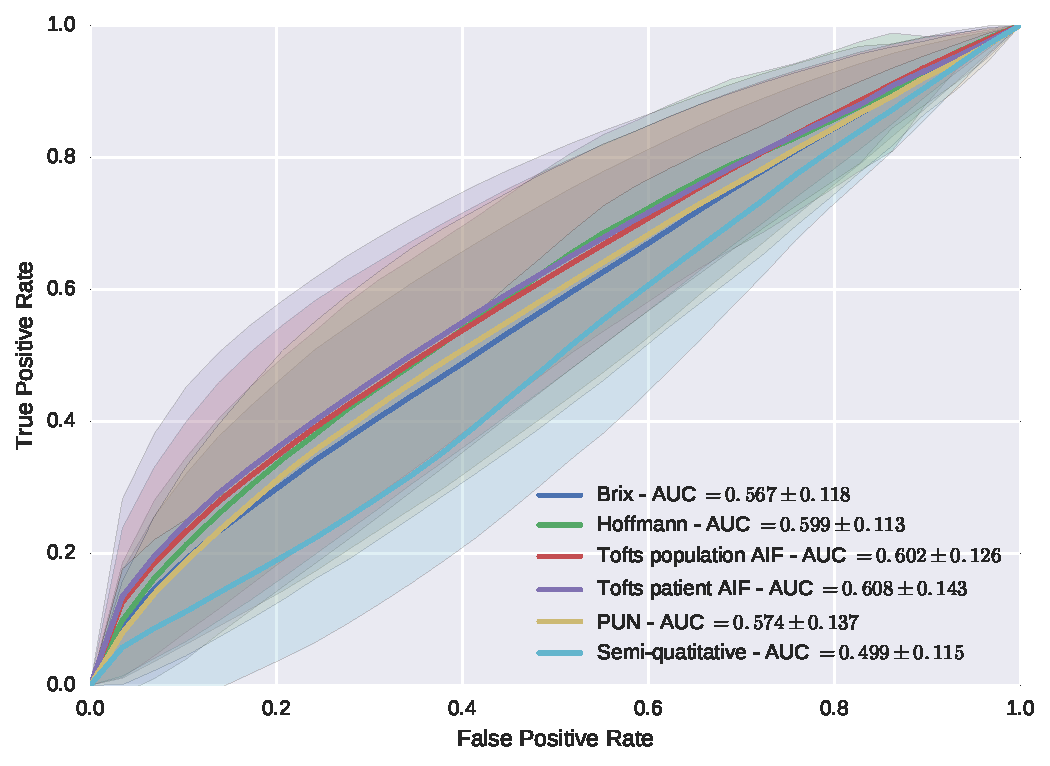
\includegraphics[width=.7\textwidth]{5_normalization/figures/DCE-normalization/unormalized_methods_0.pdf}} \\
  \subfigure[With normalization.]{\label{fig:rfpharmanorm}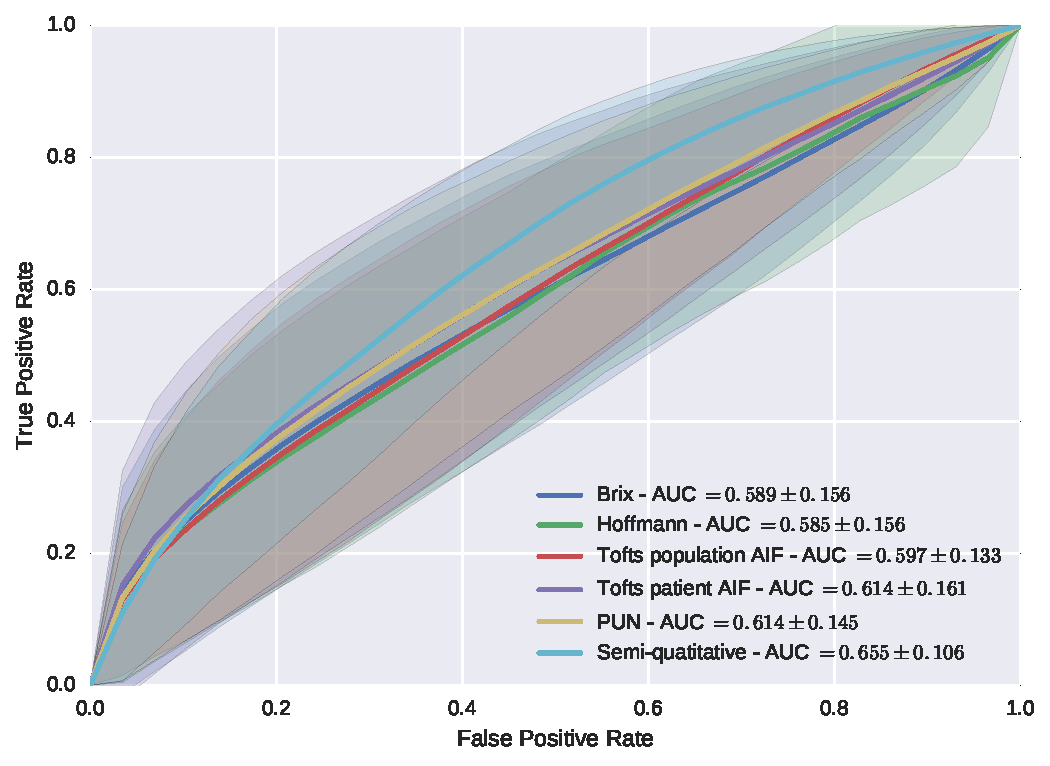
\includegraphics[width=.7\textwidth]{5_normalization/figures/DCE-normalization/normalized_methods_0.pdf}}
  \caption{\acs*{roc} analysis using a \acs*{rf} classifier (a) with and (b) without normalization of \acs*{dce}-\acs*{mri} data for different pharmacokinetic models.}
  \label{fig:normpharmarf}
\end{figure}

To study the potential benefit of our normalization, \ac{cap} are detected at a voxel level using pharmacokinetic parameters estimated from un-normalized and normalized \ac{dce}-\ac{mri} data.
Each individual pharmacokinetic parameter is classified to evaluate their individual discriminative power to detect \ac{cap}.
Therefore, a \ac{rf} classifier is used in conjunction with a \ac{lopo}.
The use of \ac{rf} is motivated since that it leads to the best performance in the state-of-the-art methods~\cite{Litjens2014,Lemaitre2015}.
Results are summarized in \acs{tab}~\ref{tab:resfeats} in terms of \ac{auc}.
Normalization can improve the detection of \ac{cap}; however, the benefit of normalization is more obvious by combining together the pharmacokinetic features of a given model --- e.g., $A$, $k_ep$, and $k_el$ for Brix model ---, as previously done in traditional \ac{cad} system~\cite{Lemaitre2015}.
For the latter configuration, results are summarized by performing a \ac{roc} analysis and computing the \ac{auc}, as reported in \acs{fig}\,\ref{fig:normpharmarf}.
Quantification using normalized data outperforms quantification using un-normalized data in terms of classification performance apart of Hoffmann and Tofts population-based \ac{aif} models.
The reasons behind the decrease of the \ac{auc} might be related to: (i) a poor fitting as discussed in \acs{sec}\,\ref{subsubsec:chp5:DCE-norm:Good} (cf., Hoffmann model) and (ii) a small number of patients while estimating some parameters (cf., Tofts model).
The best classification performance are obtained using the semi-quantitative approach with an \ac{auc} of 0.655.

\subsubsection{Classification of the entire enhanced \acs*{dce}-\acs*{mri} signal} \label{subsubsec:chp5:DCE-norm:class}

\begin{figure}
  \centering
  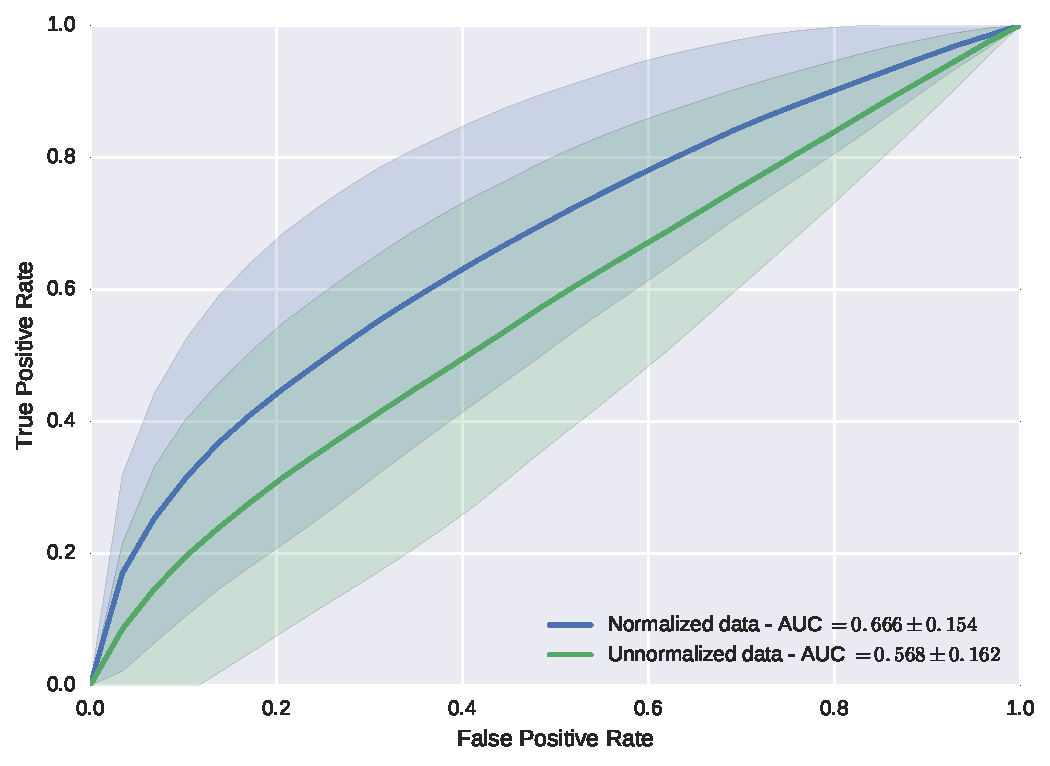
\includegraphics[width=0.7\linewidth]{5_normalization/figures/DCE-normalization/full_signal_0.pdf}
  \caption{\acs*{roc} analysis using the entire \acs*{dce}-\acs*{mri} signal with and without normalization in conjunction with a \acs*{rf} classifier.}
  \label{fig:rfnormdcesignal}
\end{figure}

As stated in the introduction, the quantification methods are extracting a set of parameters characterizing the enhancement \ac{dce}-\ac{mri} signal.
However, this extraction might lead to a loss of information.
This experiment is performed to assess if making use of the whole \ac{dce}-\ac{mri} signal instead of the just the pharmacokinetic parameters can improve the classification performance.
Therefore, each enhanced \ac{dce}-\ac{mri} signal, normalized and un-normalized, is classified using a \ac{rf} classifier in a \ac{lopo} fashion.
The \ac{roc} analysis and \ac{auc} are reported in \acs{fig}\,\ref{fig:rfnormdcesignal}.
Classification without normalization lead to the worst performance, with an \ac{auc} of 0.568.
However, data normalization in conjunction with the use of the whole \ac{dce}-\ac{mri} signal is the strategy which outperforms all others, with an \ac{auc} of 0.666.


\subsection{Discussion and conclusion}\label{subsec:chp5:DCE-norm:dis-con}

The experiments conducted in the previous section can give rise to several discussions.
In Tofts quantification, two different approaches have been used to infer the pharmacokinetic parameters: using a population-based or a patient-based \ac{aif}.
The patient-based \ac{aif} approach leads to better classification performance.
However, there are two shortcomings to take into account while advancing this fact:
(i) T$_{10}$ parameter has been fixed and not computed from a T$_1$ map and
(ii) the population-based \ac{aif} has been estimated from a cohort of only 17 patients.
These two limitations have to be considered while advancing that population-based \ac{aif} modelling is outperforming patient-based \ac{aif} modelling.

The best classification performance is reached by normalizing the \ac{dce}-\ac{mri} data and use the whole enhanced signal as feature, emphasizing the fact that a loss of information while extracting quantitative parameters.
Furthermore, this normalization is a less complex process than all quantification methods.
However, this strategy suffers from one drawback: the training time of the \ac{rf} classifier increases since that from 3 to 5 features, the feature space becomes a 40 dimensions space.

Nevertheless, this study is performed on a small cohort of patients using a single \ac{mri} machine.
Generalizing the results of this study on a larger dataset acquired from different commercial systems have to be considered to study the robustness of the proposed approach.



In this work, we presented a new method for normalizing/standardizing \ac{dce}-\ac{mri} data.
This method aimed at reducing the inter-patient variations occurring during data acquisition.
A graph-based approach was used to correct intensity offset in conjunction with a model-based correction to reduce time offset as well as intensity scaling.
We show the benefit of our normalization method prior to extract quantitative and semi-quantitative features, with a significant improvement of the classification performance.
Nevertheless, we also show that using the whole normalized \ac{dce}-\ac{mri} signal outperforms all quantitative approaches.

As avenues for future research, this normalization has to be part of a \ac{mpmri} \ac{cad} system in which \ac{dce}-\ac{mri} modality needs to be combined with other complementary modalities.
